% !TEX root = ../thesis.tex

\chapter{绪论}
\section{引言}
	在实际工程应用中,由于种种因素,如信息传输延迟、外部环境突变、子系统连接变化等,可能会导致系统结构、参数的变化。为了描述这种现象,学者们提出了Markov模型来对这类系统进行建模,并称这类系统为Markov跳变系统。近年来,由于Markov跳变系统对上述现象的强大建模能力获得了广泛而深入的研究。同时,非线性是控制系统中最常见的一类现象,在众多的非线性类别中,有一种非线性因其广泛存在及独特的结构,被学者们单独的化为一个类别,并称其为Lur'e系统。由于一些应用使用一维(1D)系统模型难以建模或模型不够精确,因而学者们提出了能更加精确建模的二维(2D)控制系统模型。在本文中,我们将围绕Markov跳变Lur'e系统、2D-Markov跳变系统展开讨论。

\section{Markov跳变系统}
	Markov跳变系统实际上是一种特殊的切换系统,当系统的结构、参数发生变化时,我们认为系统由某个子系统切换到了另一个子系统,同时,我们使用模态来表示这若干个子系统。根据这样的假设,我们不难发现,系统有多少种不同的结构、参数,就应该有多少个子系统,对应同等数量的系统模态。同其他切换系统不同的是,Markov跳变系统模态之间的切换是由一个Markov链来控制的,即模态切换遵循Markov过程。一个简单的离散Markov跳变系统\eqref{intro-system-eq}可以用图\ref{intro_system}来表示,这里$\{r(k),k\geq 0 \}$表示一个Markov链,$N$表示系统的总模态数。
	\begin{equation}\label{intro-system-eq}
		x(k+1)=A(r(k))x(k)+B(r(k))u(k)
	\end{equation}
	\begin{figure}[!htb] 
		\centering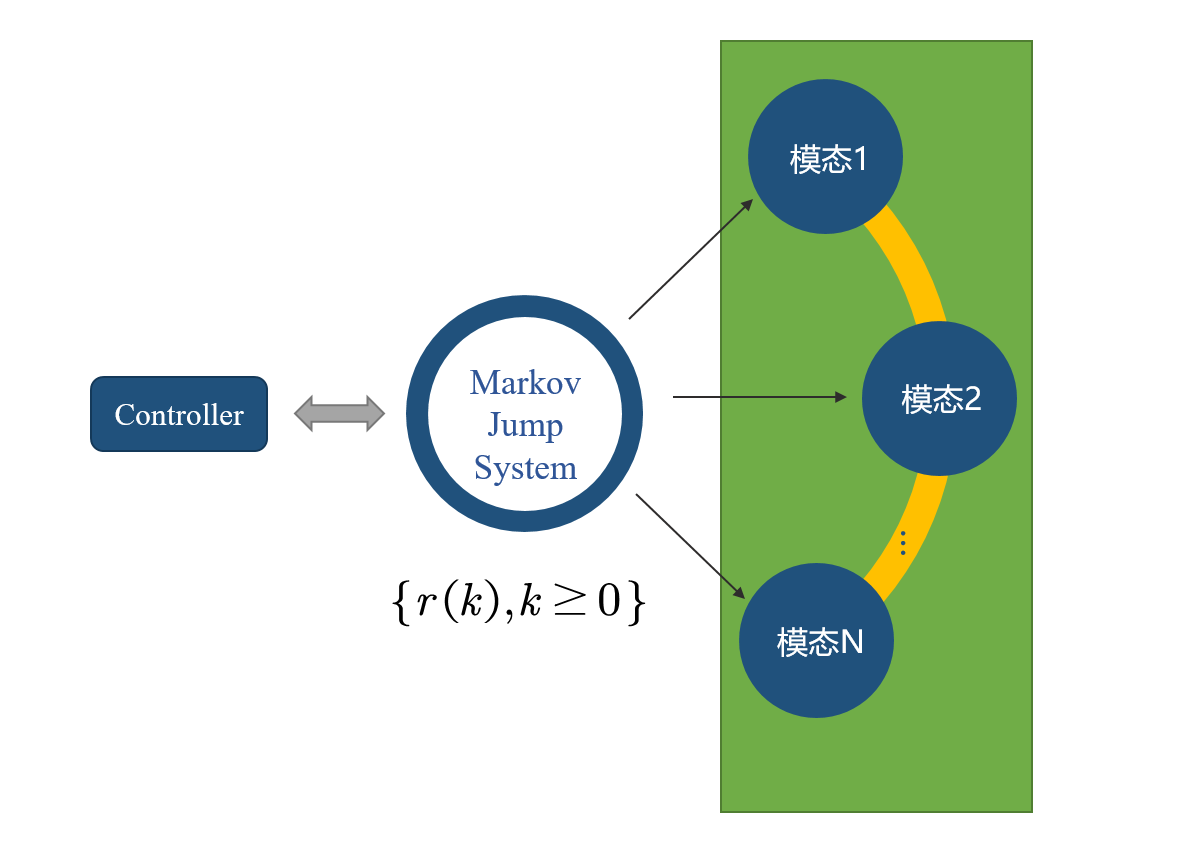
\includegraphics[scale=0.25]{./figures/introduction/system.png}\\ 
		\caption{Markov跳变系统示意图}
		\label{intro_system}
	\end{figure}

	自Markov跳变系统首次提出以来\cite{florentin1961optimal},便取得了国内外学者们的广泛关注,并取得了众多理论研究成果\cite{costa2006discrete,de2000output,xiong2005robust,ma2010stability,zhang2009hestimation,xu2007delay}。同时,Markov跳变控制系统已经成功的应用到诸如,金融分析系统\cite{mamon2007hidden}, 故障检测\cite{zhong2005faultdetection},网络通讯\cite{network-communication-kim2004},飞行器控制\cite{bar1993estimation,gray2000stability},机器臂\cite{goncalves2004nonlinear}等实际应用中。近年来,Markov跳变系统取得了诸多突破性的进展。例如,针对模态转移概率可能不确定的情况,文献\cite{zhang2009stability}提出了系统模态转移概率部分已知的控制方法,该方法涵盖了模态转移矩阵完全已知、完全未知的情况,并且利用该方法对连续、离散线性Markov跳变系统的稳定性进行了分析。之后,一些学者将该方法分别推广到了$H_{\infty}$控制\cite{luan2012h},$H_\infty$滤波\cite{ma2009robust},奇异系统\cite{kao2014stabilization}等。

\section{模态信息不匹配控制}
	目前,就Markov跳变系统,根据控制器模态同系统模态的匹配情况,可以将控制器分为三类:模态独立控制器、模态同步控制器、异步控制器。下面我们将针对这三类控制器分别展开讨论。这里,我们首先假设系统模态的模态转移概率为
	\begin{equation}\label{introduction-tps-sys}
		\Pr\{r(k+1)=j|r(k)=i \}=\pi_{ij}
	\end{equation}
	\subsection{同步控制器}
	同步控制器对应的是模态信息完全匹配的情况,一般来说,系统应该有如下形式,
	\begin{equation}
		u(k)=K(r(k))x(k)
	\end{equation}
	这里,不难发现,控制器的模态和系统的模态都是使用$r(k)$来表示的,也就是说,控制器的模态应该同系统模态保持一致,即控制器模态同系统模态完全匹配。最早关于Markov跳变系统的研究都假设控制器的模态是和系统模态保持一致的,并且取得了众多的研究成果。一般而言,模态完全匹配的情况,在系统分析上比较简单,同时,得到的结果也会比其他两种情况要好一些。但是,在实际控制系统中,控制器模态想要同系统模态始终保持一致是非常困难的。首先,由于在网络传输过程中存在信息丢失的情况,控制器可能在某些时刻获取不到系统模态信息。其次,由于网络传输存在延迟,控制器可能得到的是先前时刻的系统模态信息,而此时系统已经切换到另外一个模态,进而导致控制器模态同系统模态不匹配。另外,即使控制器及时的得到了当前时刻精确的系统模态信息,但是由于物理因素的限制,控制器可能不能及时的切换到对应模态,即控制器模态切换速度跟不上系统模态切换速度,进而又出现了模态不匹配的情况。就是说,如果想要实现模态信息始终匹配,我们需要拥有一套先进的信息传输、物理切换装置,显然,目前的科技水平是很难达到的。因此,同步控制器设计尽管分析起来非常简单,却有些不太符合实际情况了。
	
	\subsection{模态独立控制器}
	模态独立控制器对应的是模态信息完全不匹配的情况,一般来说,系统应该有如下形式,
	\begin{equation}
	u(k)=K(q(k))x(k)
	\end{equation}
	这里,$q(k)$表示控制器在$k$时刻的模态,可能在集合$\{1,2,\dots,M \}$中取值,但是服从另外一个独立的Markov过程,其状态转移概率为
	\begin{equation}\label{introdution-tps-indp}
	\Pr\{q(k+1)=j|q(k)=i \}=\lambda_{ij}
	\end{equation}
	由\eqref{introdution-tps-indp}可以推断,对模态独立控制器的情况,当前时刻的控制器模态只跟上一个时刻的控制器模态有关,同系统模态没有任何关系,即控制器模态同系统模态完全不匹配(注意,本文中,完全不匹配并不是指控制器模态始终同系统模不一致,而是两者之间不存在联系的意思)。图\ref{intro_fig_idpsys}表示了一个简单的模态独立控制器作用下的Markov跳变系统。目前,文献\cite{todorov2016new,wu2005mode,dolgov2017static}对模态独立Markov控制问题展开了研究,并得到了相应的结果。值得注意的是,当我们施加了$M=N$,$\lambda_{ij}=\pi_{ij}$,$r(0)=p(0)$这三个限制条件后,似乎控制器变成了模态完全匹配(同步)的情况,但本质上却并不是同步控制器。一个简单的理解为,假设$k$时刻系统模态和控制器模态是一样的,但是由于控制器和系统在$k+1$时刻的模态都是由概率(此时概率一样)求得的,因此也可能模态不一致,而同步控制器里,控制器在$k+1$时刻的模态是通过检测$k+1$时刻系统模态得到的。对于模态独立控制器,我们发现控制器完全没有使用到系统的模态信息,这可能导致的结果就是,最终得到的结果会比较保守,同时,在系统分析时也相对比较困难。
	
	\begin{figure}[!htb] 
		\centering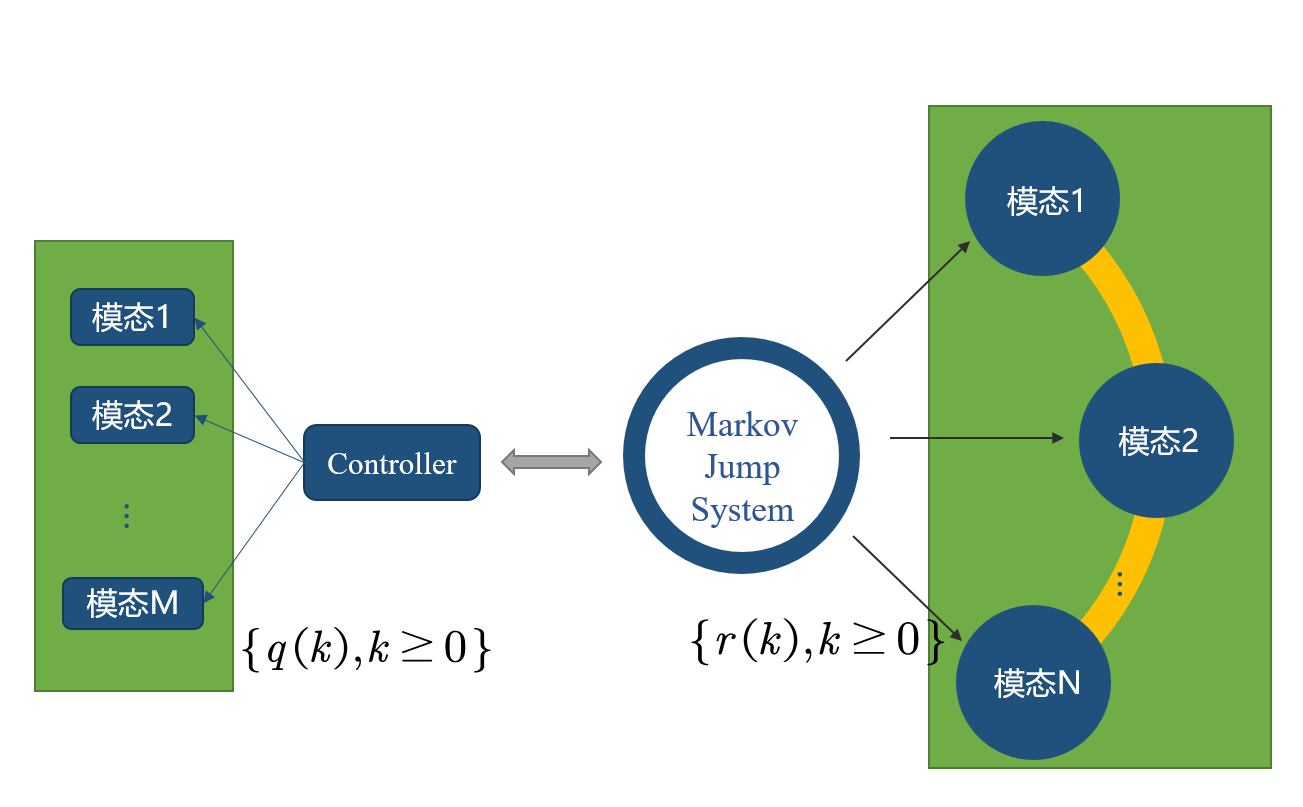
\includegraphics[scale=0.25]{./figures/introduction/idpsys.png}\\ 
		\caption{模态独立控制器作用下的Markov跳变系统}
		\label{intro_fig_idpsys}
	\end{figure}
	
	\subsection{异步控制器}
	模态独立控制器对应的是模态信息不完全匹配的情况,一般来说,系统应该有如下形式,
	\begin{equation}
	u(k)=K(\sigma(k))x(k)
	\end{equation}
	这里,$\sigma(k)$表示控制器在$k$时刻的模态,可能在集合$\{1,2,\dots,M\}$中取值,服从一个满足如下条件模态转移概率的从随机跳变过程,
	\begin{equation}\label{introdution-tps-asyn}
	\Pr\{\sigma(k)=\phi|r(k)=i \}=\mu_{i\phi}
	\end{equation}
	由\eqref{introdution-tps-asyn}我们可以发现,控制器在$k$时刻的模态是由$k$时刻的系统模态和条件概率求得的。对比同步控制器,我们可以理解同步控制器为$\mu_{ii=1}$的情况。也就是说,对同步控制器而言,$k$时刻系统模态是多少,控制器的模态就应该是多少,而对异步控制器而言,$k$时刻控制器的模态却是通过条件概率求得的,并不一定同系统模态保持一致。对比模态独立控制器,$k$时刻模态独立控制器的模态是有前一时刻($k-1$),根本就没有利用任何时刻系统的模态信息。那么,我们发现,下面几个结论(异步控制器的优点)
		
		(1) 异步控制器通过调整条件概率转变成同步控制器,
		
		(2) 异步控制器不需要严格要求控制器模态同系统模态保持一致,更符合实际情况,
		
		(3) 同模态独立控制器相比,异步控制器利用了更充分的系统信息,得到的结果更加有价值。
		
		结论(1)是比较直观的。我们重点讨论一下结论(2),这里需要注意的是,相对于同步控制器,异步控制器削弱了对同步控制器三个完美前提的依赖, 即:一定能获得系统的模态信息、系统模态信息获得足够及时、控制器在获得系统模态信息后能马上切换。异步控制器,对于上述三个前提假设,并没有采用什么优秀的改进方法来改善它们,而是正视这些不完美的存在。控制器通过一个检测器预先采集足够多的信息,统计模态间的切换规律,来推断当前控制器所处的模态。因此,在许多文章中,又称异步控制器设计方法为基于检测器的控制器设计方法。另一方面,前文中已经说过,异步控制器是基于隐Markov模型设计的,因此,基于隐Markov模型设计的控制器可以涵盖同步、异步、模态独立(1个模态)这三种情况,是一个比较综合的控制器设计方法。
	
	\begin{figure}[!htb] 
		\centering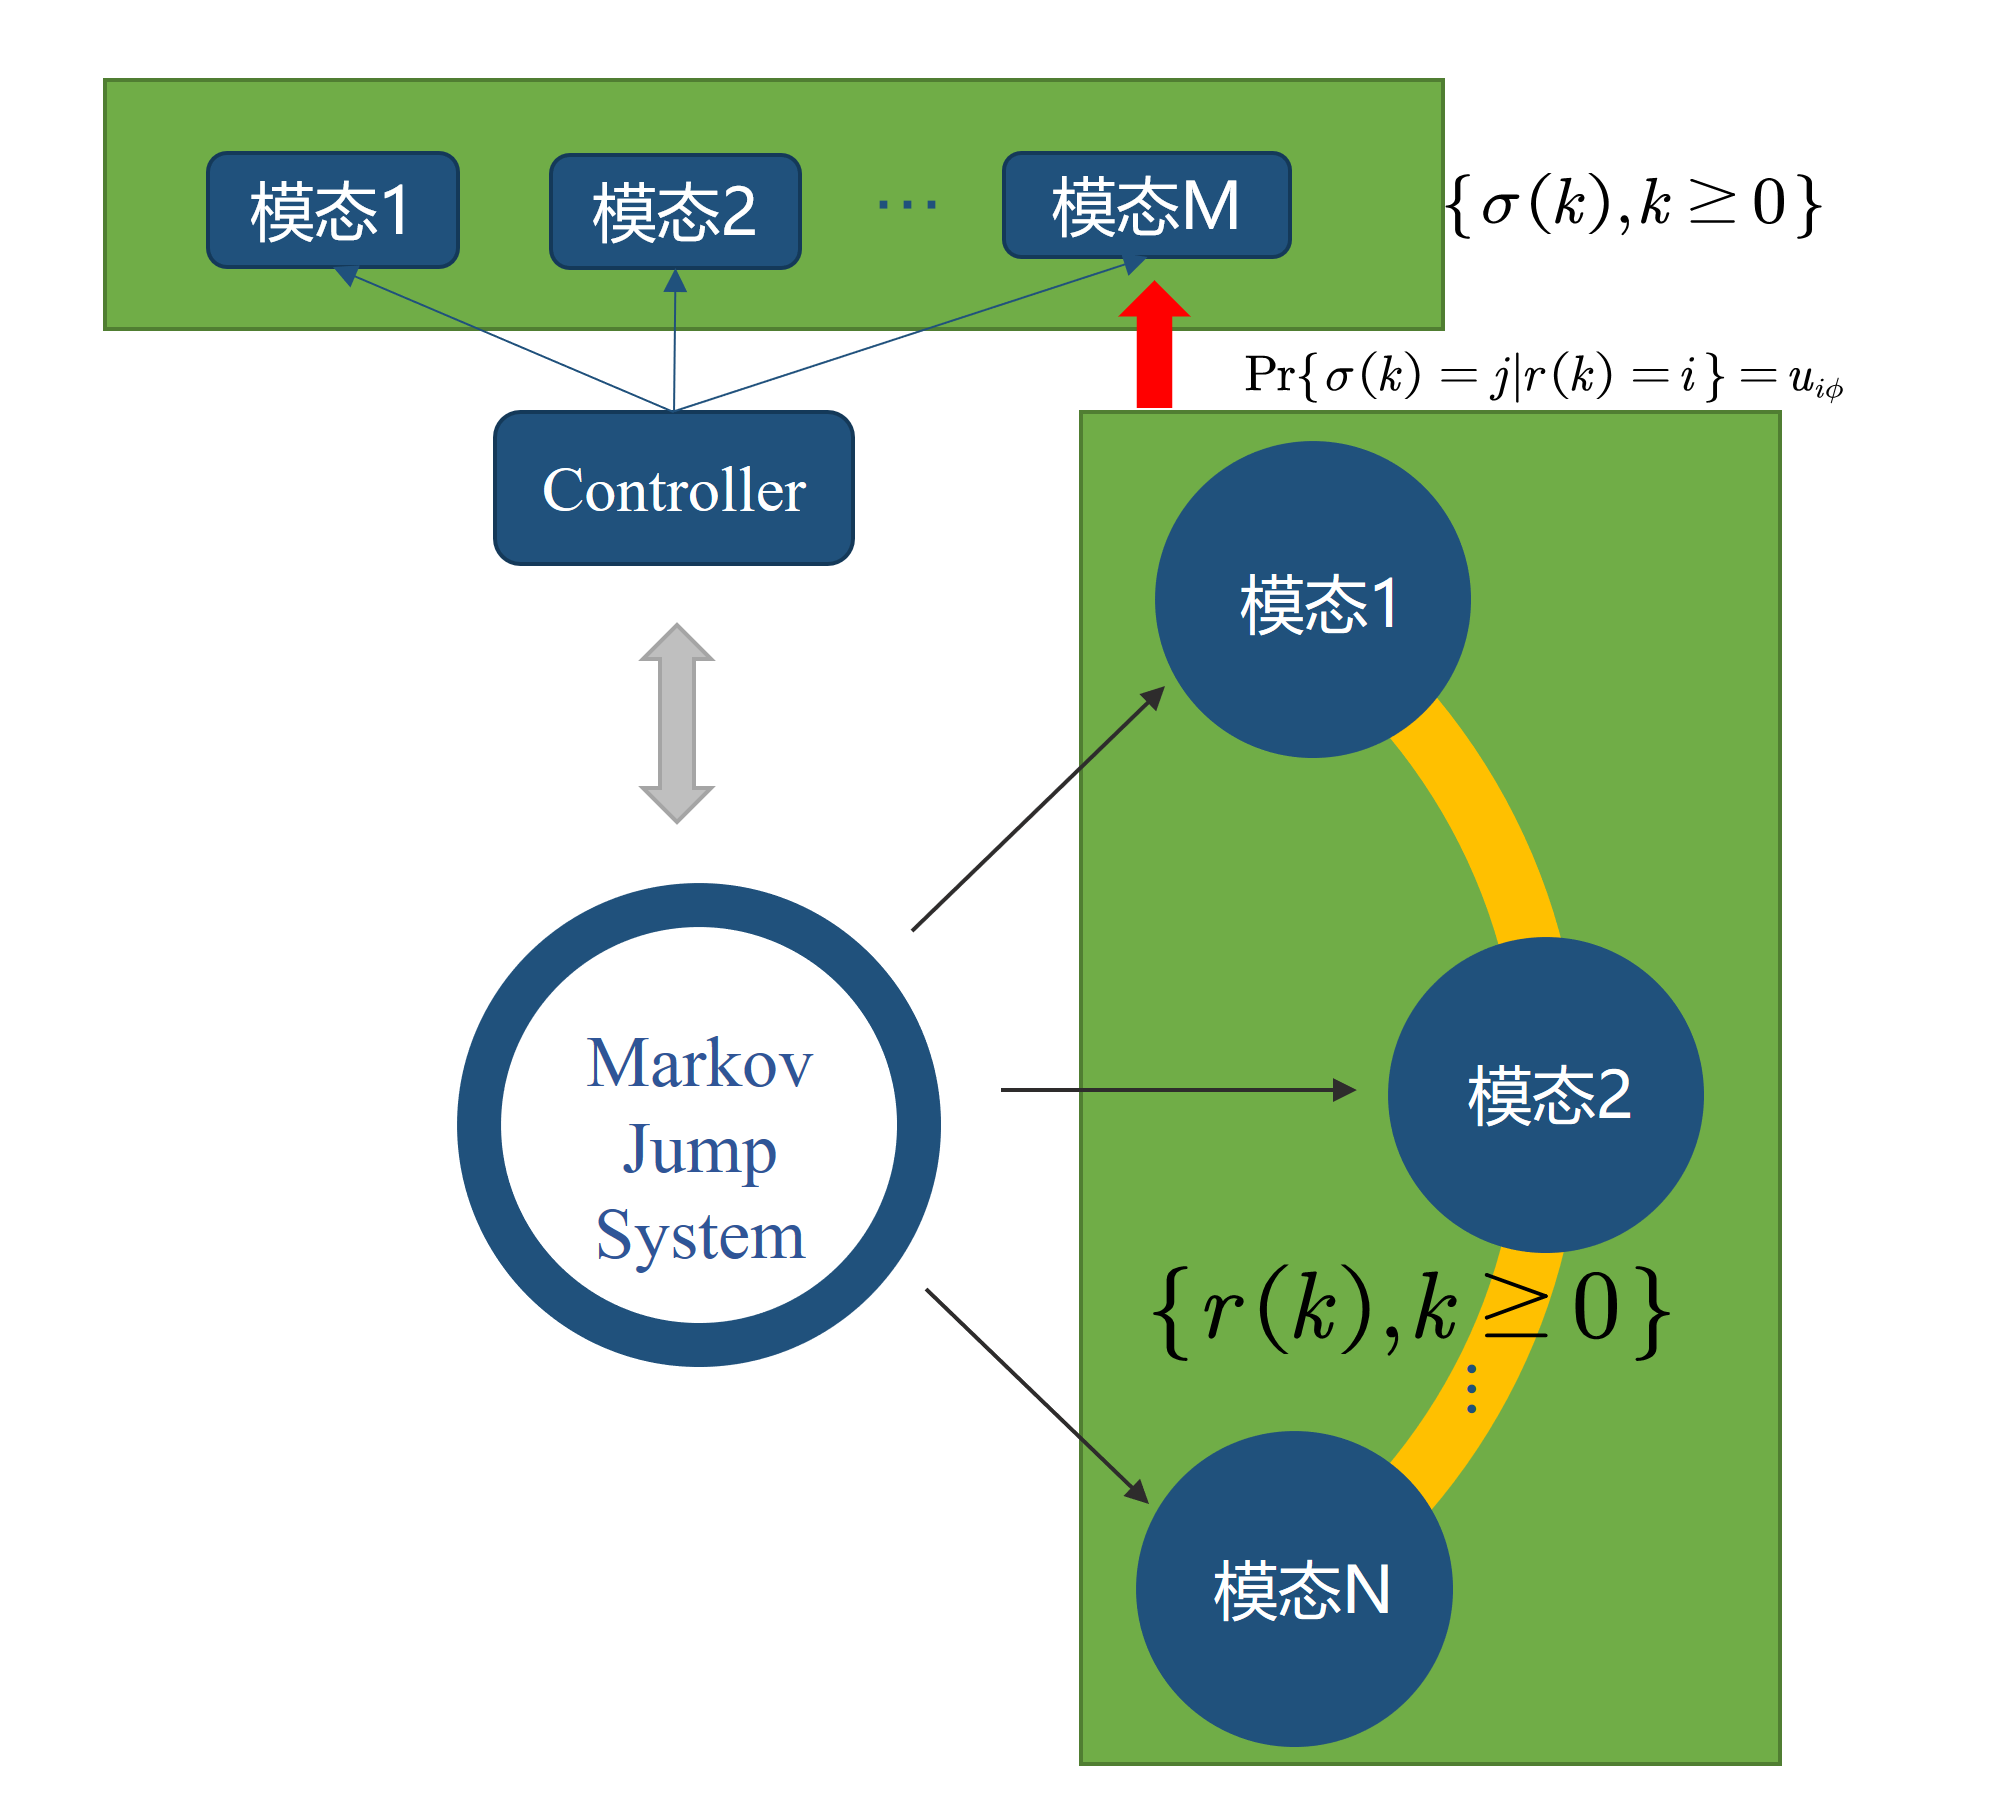
\includegraphics[scale=0.12]{./figures/introduction/asynsys.png}\\ 
		\caption{异步控制器作用下的Markov跳变系统}
		\label{intro_fig_asynsys}
	\end{figure}
	
\section{预备定理}
134
\section{本文的研究内容}
asfda